\chapter{Deep Learning}
\section{Introduction}
This final chapter of the basic current methods of classification in the text mining sector focuses very briefly on one of the newest directions called Deep Learning; see for an example, an extensive detailed book [\cite{ref103}]. This direction is inspired by the broad possibilities of artificial neural networks, which - as one might say - rank among the oldest and truly traditional algorithms.

With the rapid development of computer technology performance (speed, memory), one of the original disadvantages of neural networks - their computational demands from the hardware point of view - is gradually being overcome, opening up their further availability to wider utilization in other challenging realworld problem areas.

Which tasks are directly destined for deep learning? They typically include learning high-level attributes, or transformation of attributes, especially under the conditions when the attributes cannot be extracted or defined manually, the dimensionality of data is very high, or classical learning algorithms do not seem to work well enough or at all. Some of these conditions, if not all of them, particularly the high dimensionality apparently apply to text mining too, as the previous chapters might have suggested.

It is the characteristic of deep learning that it selects or creates relevant symptoms which may not at all be obvious to the problem being solved. The following illustration in Figure 11.1 simply illustrates the principle difference between traditional machine-learning algorithms and deep learning:

The deep learning procedure currently includes mainly multi-layer feedforward networks, deep convolutional neural networks, deep-belief networks, and recurrent neural networks for learning from sequential data.

\begin{figure}[H]
\begin{center}
  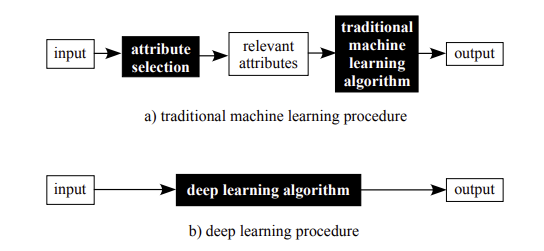
\includegraphics[width=0.8\textwidth]{chapter/chapter11/figure11_1.png}
\captionsetup{labelformat=empty}
\caption{\textbf{Figure 11.1:} Unlike the traditional machine-learning approach, deep learning selects relevant attributes (including their possible combinations) automatically.}
\label{fig11.1}
\end{center}
\end{figure}

Unfortunately, space constraints do not permit a discussion in sufficient details of all types and principles of different networks - just a description of one of them would from the material for several books. If a reader needs a deeper understanding of these algorithms, he or she can learn the details using the literature in the bibliography. Here, only one of the options using probably the most famous, basic type of artificial neural networks - feed forward network - will be briefly demonstrated. A good introduction to various types and principles of artificial neural networks can be found, inter alia, in [\cite{ref113}].

An artificial multi-layer neural network can also be viewed as a tool that can, in principle, learn hierarchically in the sense that it gradually creates attributes at higher and higher levels from attributes at lower levels, such as \textit{character} $\rightarrow$ \textit{syllable} $\rightarrow$ \textit{word} $\rightarrow$ \textit{phrase} $\rightarrow$ \textit{sentence} $\rightarrow$ \textit{paragraph} $\rightarrow$ \textit{chapter} $\rightarrow \ldots$ to attributes at higher levels based on the number of levels (defined by the user), their composition (the number and type of neurons), and the type of connection from a lower to higher level (full or sparse to reduce attributes).

Many different applications, including text mining, have already proven the great benefits of deep learning. However, it is necessary to be aware that in general, artificial neural networks count among the algorithms of the group called black-box, so it is very difficult or (almost) impossible to prove excellent classification (or regression) results by sufficient explanation, not only that "it is so," but especially "why it is so."

During their training, neural networks form very abstract spaces with virtually any number of artificial dimensions that may substantially differ from the original input dimensions. If the proper classification is sufficient for the analysis and further investigation and synthesis can be done based just on the pure classification results, no problem may arise. But if there is a need for a different justification for the results 'because the neural network has said that', then even only classifying the correct classes may not fully satisfy.

For example, in medicine, it is not enough to just diagnose - it must be justified for further correct treatment. And the same can often apply to text mining as well: Which words and phrases are relevant to a particular category? Why are the same words or phrases in several different categories? Why is something irony somewhere and not elsewhere even if the irony is almost perfectly recognized? For black-box algorithms, a wide field is still open to investigate how to justify the knowledge found.
\section{Artificial Nerual Networks}

An artificial neuron can be viewed as a transfer function $\phi($.$) having n+1$ inputs $x_i$ weighted by respective weights $w_{i}$, where $w_{i} \in \mathbb{R},-\infty<w_{i}<+\infty$ :

\begin{equation*}
\hat{y}=\phi(\mathbf{w} \cdot \mathbf{x})=\phi\left(\sum_{i=0}^{n} w_{i} x_{i}\right)=\phi\left(\theta+\sum_{i=1}^{n} w_{i} x_{i}\right), \tag{11.1}
\end{equation*}

where for the dot product of the vectors $\mathbf{w} \cdot \mathbf{x}$ with the constant value of $x_{0}=$ 1.0 there is the bias (threshold) $\theta=w_{0} x_{0}=w_{0} \cdot 1.0$ that determines the value of the transfer function $\phi($.$) from which the neuron is activated and provides its$ output $\neq 0.0$. Hence, the neuron generally makes the transformation $\mathbb{R}^{n} \rightarrow \mathbb{R}$.

Determining the specific $\phi$ function depends on the type of application and known or anticipated properties of the approximated unknown function $\hat{y}=\hat{f}(\mathbf{x})$. A commonly used nonlinear transfer function $\phi$ is sigmoid (known also as logistic), $S(x)$, where

$$
S(x)=\left(1+e^{-1}\right), \lim _{x \rightarrow-\infty} S(x)=0, \lim _{x \rightarrow+\infty} S(x)=1,
$$

and where, for classification, the usual threshold when the neuron returns 1 is for $S(x) \geq 0.5$, otherwise 0 . However, there are also a number of alternatives required usually by specific applications for certain reasons; details can be found in literature.

Neurons can be combined in layers into a network to approximate unknown complex nonlinear (including discontinuous or non-differentiable) functions, which can also be used advantageously for classification or regression. The error function $E$ of the approximation (or classification in our case) is usually defined as follows:


\begin{equation*}
E=\frac{1}{2}(y-\hat{y})^{2}, \tag{11.2}
\end{equation*}


where $y$ is a known correct value and $\hat{y}$ is a value returned for the given training data sample by the trained network. The square of the difference $y-\hat{y}$ eliminates negative error values and highlights larger errors whose removal takes precedence over smaller errors (multiplication by $\frac{1}{2}$ is just for formal reasons, so\\
that the number 2 in the exponent may not be considered in the derivative when looking for the steepest descent of the error).

To correct the output of $\phi(\mathbf{w} \cdot \mathbf{x})$ for the input sample $\mathbf{x}$, only the weight vector $\mathbf{w}$ can be modified because the values of $\mathbf{x}$ are given. This modification affects the significance of the $n$ weighted individual components (attributes $x_{i}$ ) of the input vector $\mathbf{x}=\left(x_{1}, x_{2}, \ldots, x_{n}\right)$, the combination of which determines the required output value of the approximated function $\hat{f}(\mathbf{x})$.

Of course, no weights $w_{i}$ are known before starting the training process. These weights always determine the instantaneous position of a point representing a certain iterative solution in an $n$-dimensional space.

The goal is ideally the optimal solution - in our case, the maximal classification accuracy (alternatively the minimum classification error), which is the global maximum of the desired function $\hat{f}(\mathbf{x}) \approx f \mathbf{x}$ ).

The initial $w_{i}$ 's values define the starting point and because it is typically not known where to start from, it is only possible to randomly generate those coordinate values. In a case when there would be some initial, if limited, knowledge available, it would be possible to determine the starting subspace (or point) more precisely.

Due to possible error on the trained network's output, it is necessary to appropriately adjust the weights of the attributes. In each iteration step, it is commonly gradually done for the individual layers in the direction from the output to the input layer - therefore the term 'backup error propagation' is often used. All the necessary detail can be found in, for example, [113], or other existing literature.

\begin{figure}[H]
\begin{center}
  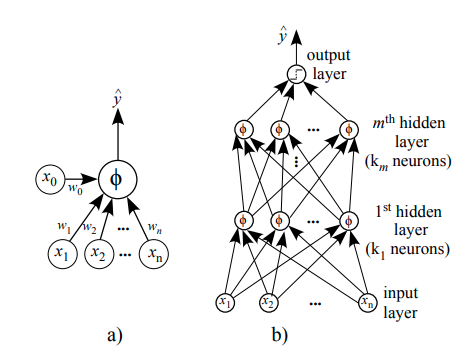
\includegraphics[width=0.8\textwidth]{chapter/chapter11/figure11_2.png}
\captionsetup{labelformat=empty}
\caption{\textbf{Figure 11.2:} An artificial neuron (a) and a multi-layer feed-forward classification neural network composed of neurons (thresholds are omitted) (b).}
\label{fig11_2}
\end{center}
\end{figure}

\begin{figure}[H]
\begin{center}
  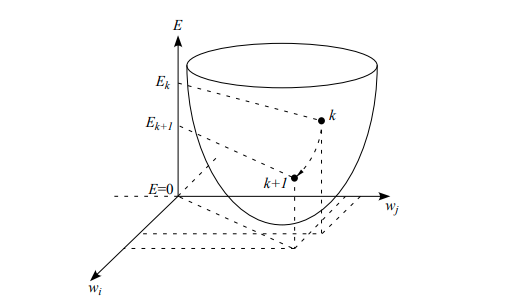
\includegraphics[width=0.8\textwidth]{chapter/chapter11/figure11_3.png}
\captionsetup{labelformat=empty}
\caption{\textbf{Figure 11.3:} At an iteration step $k$, the steepest descent across the surface of the error function, $E$, is found and the coordinates (weights) of the point position are corrected so that it moves towards the lower error value at $k+1$.}
\label{fig11_3}
\end{center}
\end{figure}

In fact, it is about converting the original space described by the vectors $\mathbf{x}$ into a highly different abstract space described by the vectors $\mathbf{w}$, which typically has many more artificially introduced dimensions (transformed attributes). In this new space, the neural network is looking for (and often successfully finds) the desired approximated solution.

Note that generally non-linear functions may suffer from having a lot of local extremes where it is easy to get stuck in finding the global extreme. If the idea of searching for the highest mountain in the misty, heavily mountainous landscape is used, then it is obvious that success can depend on the location from which the search begins - far from or near the foot of the highest mountain.

Therefore, it is advisable to search repeatedly from different starting points and compare the achieved results, which can be done by a newly generated set of the coordinates using different random-generator seeds.

If these results are the same or very similar, then it is very probable that the best achievable solution was found.

\section{Deep Learning in R}

Today, a lot of freely accessible software tools implementing various artificial neural networks are available. The tools commonly include many useful acceleration and optimization enhancements from both the mathematical and implementation point of view. In addition, there are still upcoming new enhancements
or new types of neural networks, so the selection is fairly wide and the user can also choose from the task type being solved.

The R-language add-on system is no exception, and a variety of methods and algorithms can be found, sometimes more general, sometimes tailor-made for specific task groups. For ease of use and installation, this chapter confines itself to demonstrating the use of a single artificial neural network system - SNNS, which stands for Stuttgart Neural Network Simulator, one of the outstanding simulation systems [\cite{ref287}].

The SNNS is called as a function $mlp()$ with the main parameters size $=c(1000,500,200,80,20)$ defining gradually the individual layer sizes from the network input to its output, and maxit=50 defining the number of iterations.

\begin{verbatim}
library(Rcpp)
library(RSNNS)
# loading the data
data <- read.csv("BookReviews.csv", header=TRUE)
# converting the data to a matrix
dtm <- as.matrix(data)
# removing the object data (unnecessary from now)
rm(data)
# number of instances
n <- dim(dtm)[1]
# number of attributes
m <- dim(dtm)[2]
# indexes of 100 testing samples
number_of_test_samples <- 100
test_index <- 1:number_of_test_samples
# selecting training samples
train_data <- dtm[-test_index, 1:(m-1)]
train_labels <- dtm[-test_index, m]
# selecting testing samples
test_data <- dtm[test_index, 1:(m-1)]
test_labels <- dtm[test_index, m]
# training a neural network model
\end{verbatim}

\begin{verbatim}
rsnns_model <- mlp(train_data, train_labels,
        size=c(1000, 500, 200, 80, 20),
        learnFuncParams=c(0.1),
        maxit=50)
# plotting iterative errors of the rsnns_model object
plotIterativeError(rsnns_model, main="Iterative error")
# plotting a ROC curve for training data
plotROC(fitted.values(rsnns_model),
    train_labels,
    main="ROC curve - training data",
    xlab="1 - specificity",
    ylab="sensitivity")
# calculating class predictions for test data
predictions <- predict(rsnns_model, test_data)
# plotting a ROC curve for test data
plotROC(predictions,
    test_labels,
    main="ROC curve - test data",
    xlab="1 - specificity",
    ylab="sensitivity")
# creating a confusion matrix for training data (label 1
# is assigned when the output value > 0.6 and the remaining
# outputs are less than 0.4)
print(confusionMatrix(
    train_labels,
    encodeClassLabels(fitted.values(rsnns_model),
            method="402040",
            l=0.4, h=0.6)))
# transforming real numbers to 0 or 1
predictions <- round(predictions)
# creating a confusion matrix
cm <- table(test_labels, predictions)
print("Confusion matrix")
print(cm)
\end{verbatim}

\begin{verbatim}
# number of instances
n <- sum(cm)
# number of correctly classified instances for each class
correct <- diag(cm)
# numbers of instances in each class
instances_in_classes <- apply(cm, 1, sum)
# numbers of each class predictions
class_predictions <- apply(cm, 2, sum)
# accuracy
accuracy <- sum(correct)/n
# precision per class
precision <- correct/class_predictions
# recall per class
recall <- correct/instances_in_classes
# F1-measure per class
f1 <- 2 * precision * recall / (precision + recall)
# printing summary information for all classes
df <- data.frame(precision, recall, f1)
print("Detailed classification metrics")
print(df)
print(paste("Accuracy:", accuracy))
# macroaveraging
print("Macro-averaged metrics")
print(colMeans(df))
# microaveraging
print("Micro-averaged metrics")
print(apply(df, 2, function (x)
    weighted.mean(x, w=instances_in_classes)))
\end{verbatim}

For the demonstrated classification example, the console gives the following textual output that contains the confusion matrix for training samples, a con-\\
fusion matrix for testing samples, and the classification performance values for positive, negative, and all training samples:

\begin{flushleft}
\texttt{predictions} \\
\begin{tabular}{lrr}
                   & 0 & 1 \\
targets 0 & 434 & 9   \\
1         & 2   & 455 \\
\end{tabular}

\texttt{[1] "Confusion matrix"} \\
\texttt{predictions} \\
\begin{tabular}{lrr}
                           & 0 & 1 \\
test\_labels 0 & 40  & 17  \\
1             & 4   & 39  \\
\end{tabular}

\texttt{[1] "Detailed classification metrics"} \\
\begin{tabular}{lrrr}
  & precision & recall & f1 \\
0 & 0.9090909 & 0.7017544 & 0.7920792 \\
1 & 0.6964286 & 0.9069767 & 0.7878788 \\
\end{tabular}

\texttt{[1] "Accuracy: 0.79"}

\texttt{[1] "Macro-averaged metrics"} \\
\begin{tabular}{rrr}
precision & recall & f1 \\
0.8027597 & 0.8043656 & 0.7899790 \\
\end{tabular}

\texttt{[1] "Micro-averaged metrics"} \\
\begin{tabular}{rrr}
precision & recall & f1 \\
0.8176461 & 0.7900000 & 0.7902730 \\
\end{tabular}
\end{flushleft}

In addition, three graphs are available. The first grapf, Figure 11.4, represents the decrease of the sum of squared errors $(y-\hat{y})^{2}$, SSE, during the iteration process. It clearly illustrates how the network learns.

The next graph, Figure 11.5, shows the dependence of the so called sensitivity value on the specificity value for the training data, while the third graph, Figure 11.6, shows the same for the test data. Sensitivity (or recall) is also known as true positive rate, $T P /(T P+F N)$, while specificity is known as true negative rate, $T N /(F P+T N)$.

Alternatively, this dependence can be also used to express the relative relationship between the positive examples mistaken for negative and negative ones mistaken for positive. Such a dependence function may be useful for visual comparison of classifier behaviour on test and training examples. The presented neural network learned the training samples almost perfectly for both classes while the testing samples gave more errors. However, it can be usually expected.

\begin{figure}[!ht]
\begin{center}
  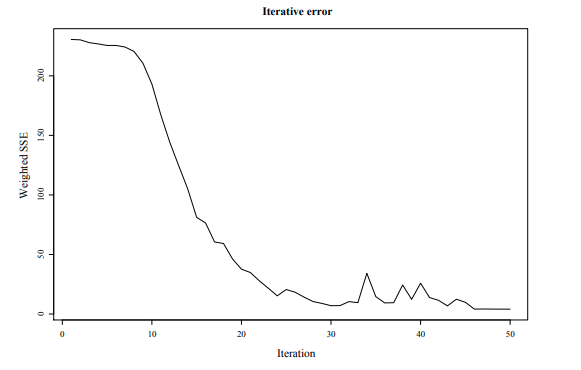
\includegraphics[width=0.8\textwidth]{chapter/chapter11/figure11_4.png}
\captionsetup{labelformat=empty}
\caption{\textbf{Figure 11.4:} The squared sum of error decrease depending on an iteration step number during learning.}
\label{fig11.4}
\end{center}
\end{figure}

\begin{figure}[!ht]
\begin{center}
  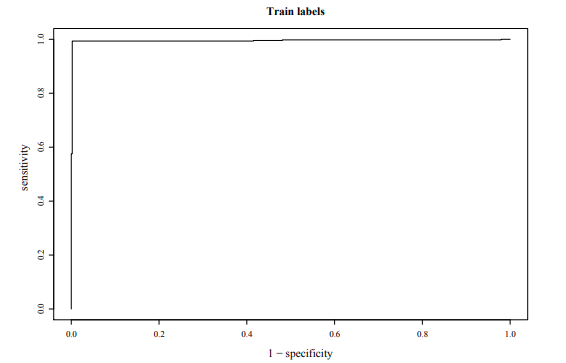
\includegraphics[width=0.8\textwidth]{chapter/chapter11/figure11_5.png}
\captionsetup{labelformat=empty}
\caption{\textbf{Figure 11.5:} The dependence between the positive samples mistaken for negative and negative ones mistaken for positive (training samples).}
\label{fig11.5}
\end{center}
\end{figure}

\begin{figure}[H]
\begin{center}
  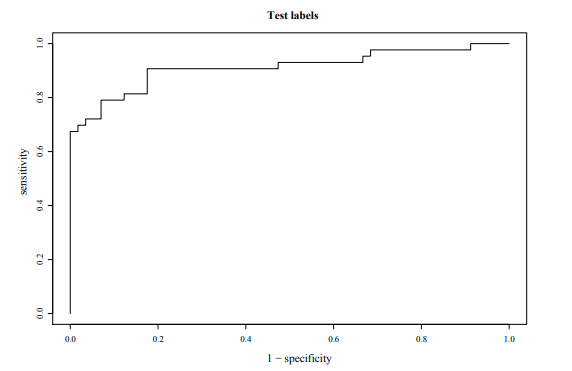
\includegraphics[width=0.8\textwidth]{chapter/chapter11/figure11_6.png}
\captionsetup{labelformat=empty}
\caption{\textbf{Figure 11.6:} The dependence between the positive samples mistaken for negative and negative ones mistaken for positive (test samples).}
\label{fig11.6}
\end{center}
\end{figure}

The applied software package, RSNNS, is only one possibility for deep learning. There are also other popular packages that can be applied. One of the popular alternative packages which was originally developed for another programming language, Python, is known under the name keras. However, the machine learning community also enabled the use of keras for R ; thus, it is freely available in R as well, including an R interface.

The referenced keras system is very rich in terms of usable features and parameters, so it is worth paying attention to the appropriate accessible documentation available, to a large extent (in various forms, with different content) via the Internet - unfortunately, space restrictions do not allow for more details here. An interested user may start from [\cite{ref50}, \cite{ref10}, \cite{ref83}] and continue with other references offered in available resources.

% \include{sublogo}